
\chapter{Energia di Coesione e Classificazione dei Solidi}

\section{Classificazione dei Solidi}

A differenza del capitolo precedente, in cui i solidi sono stati descritti principalmente in base alla struttura geometrica, in questo capitolo si classificheranno i solidi in base alla configurazione degli elettroni in valenza.  
La distinzione principale viene fatta tra metalli e isolanti e si basa sulla distribuzione elettronica nello spazio $k$.  
Nei metalli si osserva la presenza di bande semipiene, mentre negli isolanti gli elettroni risultano fortemente localizzati.

\subsection{Isolanti}
Gli isolanti possono essere classificati in tre gruppi:
\begin{itemize}
    \item \textbf{Cristalli covalenti:} in cui la distribuzione elettronica è molto localizzata lungo direzioni ben definite, legata alla formazione dei legami covalenti.
    \item \textbf{Cristalli molecolari:} per esempio, i gas nobili allo stato solido, caratterizzati da shell elettroniche completamente piene.
    \item \textbf{Cristalli ionici:} dove l'interazione principale è di natura coulombiana, dovuta alla presenza di ioni.
\end{itemize}

\subsection{Cristalli Alogenuro-Alcalini}
I cristalli alogenuro-alcalini sono cristalli ionici formati da un catione (tipicamente un metallo alcalino) e un anione (tipicamente un alogeno).  
La stabilità di tali solidi è dovuta al potenziale coulombiano che si instaura tra ioni di carica opposta.  
Per fare un esempio, consideriamo il cristallo di \ce{RbBr}:  \\
per formare uno ione \ce{Br-} è necessaria un'energia di circa \SI{-3.5}{\electronvolt}, mentre per formare uno ione \ce{Rb+} occorrono circa \SI{4.2}{\electronvolt}.  
Apparentemente, un atomo di Rb legato a un atomo di Br implicherebbe un consumo netto di energia di circa \SI{0.5}{\electronvolt}.  
Tuttavia, abbassando la distanza tra gli ioni, l'interazione elettrostatica riduce significativamente l'energia, così che nel cristallo \ce{RbBr}, per una distanza tipica di $r \approx$ \SI{0.34}{\nano\meter}, l'energia coulombiana raggiunge valori di circa \SI{-4.2}{\electronvolt}, compensando ampiamente il contributo energetico positivo.\\
La struttura reticolare dei cristalli alogenuro-alcalini è confermata anche da diffrazioni a raggi X.  
In Figura \ref{fig:NaCl-cristallo} è riportata la densità di carica elettronica per il caso dell'\ce{NaCl}.
\begin{figure}[H]
    \centering
    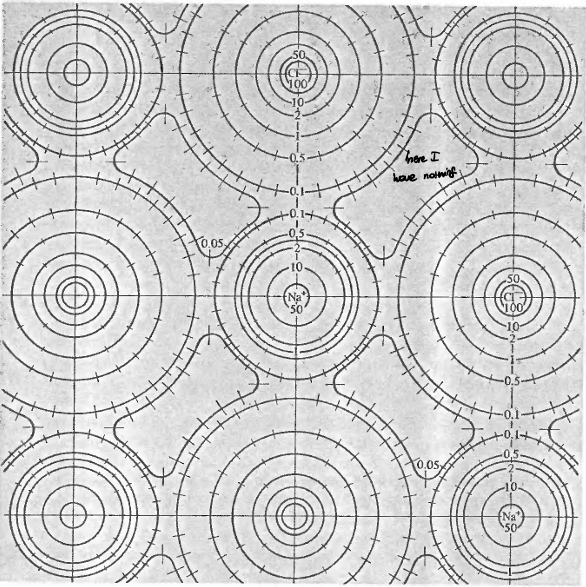
\includegraphics[width=0.5\textwidth]{images/7-Classificazione-Solidi/cristNaCl.png}
    \caption{Densità di carica elettronica nell'NaCl.}
    \label{fig:NaCl-cristallo}
\end{figure}

Dal punto di vista elettronico, essendo degli isolanti, questi cristalli presentano un ampio gap tra la banda di valenza e quella di conduzione.  
Inoltre le bande sono molto piatte, il che implica che la derivata seconda dell'energia rispetto al vettore d'onda è piccola.  
Questo porta a una massa efficace elevata e, conseguentemente, a una bassa mobilità degli elettroni, come si evince dal grafico in Figura \ref{fig:bande-alk-hal}.

\begin{figure}[H]
    \centering
    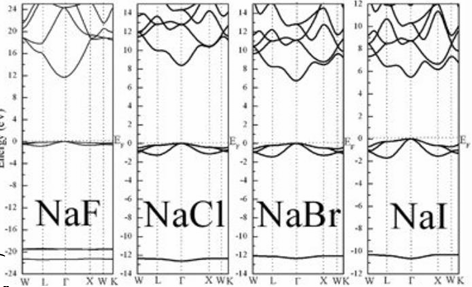
\includegraphics[width=0.5\textwidth]{images/7-Classificazione-Solidi/bandealkhal.png}
    \caption{Bande elettroniche nei cristalli alogenuro-alcalini: bande piatte che indicano una bassa mobilità elettronica.}
    \label{fig:bande-alk-hal}
\end{figure}

\noindent
Confrontando la distanza tra due ioni in un cristallo ionico con la metà della distanza tra il primo vicino in un metallo (vedi Figura \ref{fig:dist-metalli}), si osserva che nei cristalli ionici gli ioni sono molto più vicini tra loro rispetto agli atomi in un metallo.  
Questo fatto solleva il problema: \emph{che cosa tiene insieme un metallo?}  
La risposta risiede negli effetti puramente quantistici derivanti dall'interazione degli elettroni, che stabilizzano il reticolo metallico anche se gli atomi sono più distanziati.

\begin{figure}[H]
    \centering
    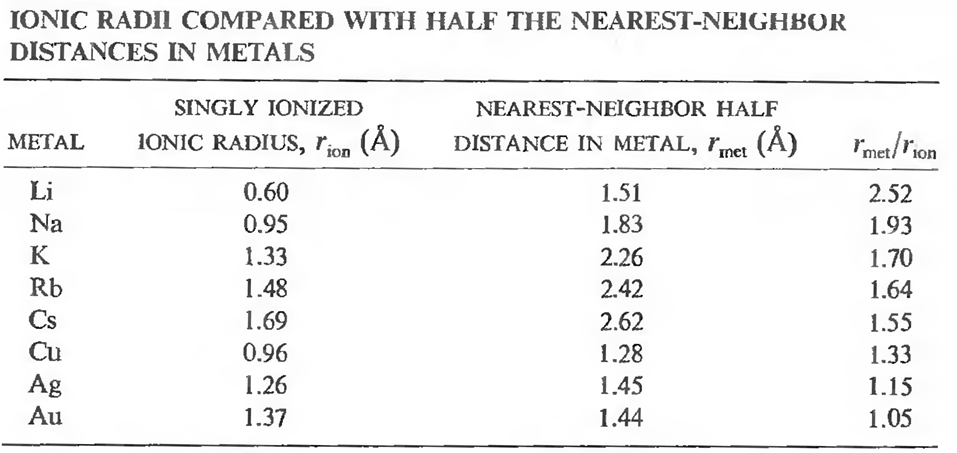
\includegraphics[width=0.8\textwidth]{images/7-Classificazione-Solidi/Distmetalli.png}
    \caption{Confronto tra le distanze interatomiche nei metalli e negli ioni in un cristallo ionico.}
    \label{fig:dist-metalli}
\end{figure}


\section{Energia di Coesione}
L'energia di coesione è l'energia necessaria per estrarre un atomo dal cristallo, vediamo l'energia di coesione nei diversi tipi di solido.
\subsection{Forze di Van Der Waals e potenziale di Lennard-Jones}
Le forze di Van der Waals sono forze di attrazione o repulsione deboli che si manifestano tra molecole (o atomi) neutri, non legate da legami chimici covalenti o ionici. Sono fondamentali per spiegare molti fenomeni fisici e chimici, come la condensazione dei gas, la coesione tra molecole nei liquidi e il comportamento delle molecole biologiche.\\\\
Come si orginano? Supponiamo di avere due atomi ad una distanza $r$, anche se la loro distribuzione di carica media è simmetrica, possiamo avere fluttuazioni istantanee che genererano un momento di dipolo istantaneo $p_1$ con un campo elettrico $E \propto \frac{p_1}{r^3}$. Quest'ultimo a sua volta indurrà un momento di dipolo istantaneo nell'atomo 2 che sarà pari a $ p_2 = \alpha E \sim \frac{\alpha p_1}{r^3}$, con $\alpha$ polarizzabilità, ossia la misura della deformazione di carica.\\
L'energia potenziale dovuta all'interazione tra i due dipoli sarà data da:
\[ \frac{p_2 p_1}{r^2} \sim \frac{\alpha p_1^2}{r^6}\]
Dimostriamolo usando la meccanica quantistica: \\
considera la situazione riportata in Figura \ref{fig:dip}
\begin{figure} [H]
    \centering
    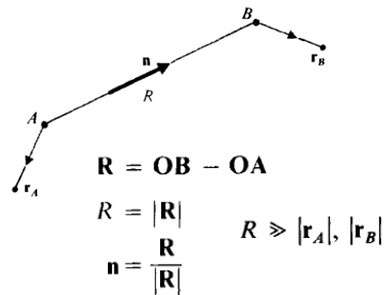
\includegraphics[width=0.5\textwidth]{images/7-Classificazione-Solidi/dip.png}
    \caption{}
    \label{fig:dip}
\end{figure} 

Il dipolo è dato da:
\[ \begin{split}
    &\mathcal{D}_A = qr_A \\
    &\mathcal{D}_B = qr_B \\
\end{split}\]
L'energia potenziale di un dipolo in un campo elettrico è:
\[ U(\mathbf{R}) = \frac{1}{4\pi\varepsilon_0} \frac{\mathcal{D}_A\cdot \mathbf{R}}{R^3}\]
Quindi:
\[ \mathbf{E} = -\nabla_R U = -\frac{q}{4\pi\varepsilon_0}\frac{1}{R^3}[\mathbf{r}_A-3(\mathbf{r}_A \cdot \mathbf{n})\mathbf{n}]\]
ora andiamo a vedere l'interazione del campo elettrico generato dal dipolo $\mathcal{D}_A$ con il dipolo $\mathcal{D}_B$, quindi dato $r_{A,B} = x_{A,B} \hat{i}+y_{A,B}\hat{j}+z_{A,B}\hat{k}$ otteniamo:
\[
\begin{split}
    &\mathcal{W}_{dd} = - \mathbf{E} \cdot \mathcal{D}_B = \frac{e^2}{R^3}[ \mathbf{r}_A \cdot \mathbf{r}_B - 3(\mathbf{r}_A \cdot \mathbf{n})(\mathbf{r}_B \cdot \mathbf{n})] \\
    & \implies \mathcal{W}_{dd} = \frac{e^2}{R^3}(x_Ax_B + y_Ay_B - 2z_Az_B)
\end{split}
\]
Ora trasformiamo questo approccio classico in un operatore quantistico
\begin{equation}
    \mathcal{W}_{dd} = \frac{e^2}{R^3} (X_AX_B + Y_AY_B -2Z_AZ_B)
    \label{eqn:quantum-wdd}
\end{equation}
dove in questo caso $X$ è l'operatore posizione associato al dipolo. L'hamiltoniana sarà: 
\[H = H_{0A}+H_{0B} + \mathcal{W}_{dd}\]
dove le $H_0$ sono le hamiltoniane atomiche e $\mathcal{W}_{dd}$ è la parte di interazione, quindi utilizzo la teoria delle perturbazioni:
\[(H_{0A}+H_{0B})\ket{\psi_{n,l,m}^A; \psi_{n',l',m'}^B} = (E_n + E_{n'})\ket{\psi_{n,l,m}^A; \psi_{n',l',m'}^B} \]
Allo stato fondamentale imperturbato l'energia sarà la somma dell'energia dei due stati fondamentali dei due singoli atomi $E_T = -2E_0$.\\
Mentre la perturbazione al primo ordine sarà:
\[ \varepsilon_1 = \bra{\psi_{1,0,0}^A;\psi_{1,0,0}^B}\mathcal{W}_{dd}\ket{\psi_{1,0,0}^A;\psi_{1,0,0}^B} = 0\]
Questo perché è il prodotto dei termini \\
\[\bra{\psi_{1,0,0}^A;\psi_{1,0,0}^B} X_A \ket{\psi_{1,0,0}^A;\psi_{1,0,0}^B}\bra{\psi_{1,0,0}^A;\psi_{1,0,0}^B}X_B\ket{\psi_{1,0,0}^A;\psi_{1,0,0}^B} = 0\]
in quanto allo stato stazionario il  valore medio delle componenti degli operatori di posizione è zero.\\
Quindi dobbiamo andare al secondo ordine:
\begin{equation*}
\varepsilon_2 = \sum_{\substack{n,l,m \\ n',l',m'}} \frac{|\bra{\psi_{n,l,m}^A;\psi_{n',l',m'}^B} \mathcal{W}_{dd}\ket{\psi_{1,0,0}^A;\psi_{1,0,0}^B}|^2}{-2E_1-E_n-E_{n'}}
\end{equation*}
data (\ref{eqn:quantum-wdd}) estraggo $\left| \frac{1}{R^3} \right|^2$ dalla somma e ottengo:
\[ \varepsilon_2 = - \frac{C}{R^6}\]
dove C è il numero che sarà dato da $\bra{...}\mathcal{W}_{dd}\ket{...}$ senza $1/R^3$. \\
\textbf{Quindi possiamo concludere che le forze di Van der Waals sono di tipo attrattivo (segno meno) e sono date dal secondo ordine perturbativo dell'energia.}
\\~\\
Quando gli atomi si avvicinano però entra in gioco la repulsione dei nuclei atomici, quindi il potenziale che descrive al meglio il sistema in modo più semplice possibile è quello di \textbf{Lennard-Jones} (Figura \ref{fig:lennard-jones}). La relazione che descrive questo potenziale è stata ottenuta tramite  un approccio semi empirico fittando dati sperimentali
\[ \phi(r) = -\frac{A}{r^6} + \frac{B}{r^{12}}\]
dove il primo termine indica l'attrazione dovuta alle forze di Van der Waals e il secondo è la repulsione dei nuclei. Il fatto che sia alla 12esima potenzia il termine repulsivo non ha alcun significato fisico, viene dal fit ed è arbitrario, semplicemente serviva qualcosa che divergesse velocemente su piccole distanze. \\
Un altro modo per scrivere questa relazione è:
\begin{equation}
\begin{split}
 &\phi(r) = 4\varepsilon \left[ \left( \frac{\sigma}{r}\right)^{12} - \left( \frac{\sigma}{r}\right)^6 \right] \\
 & \sigma = \left( \frac{B}{A}\right)^{\frac{1}{6}} \\
 & \varepsilon = \frac{A^2}{4B}
\end{split}
\label{eqn:lennard-jones-pot}
\end{equation}
dove $\varepsilon$ è un parametro che ha le dimensioni di un'energia ed è relativo all'energia di coesione mentre $\sigma$ ha le dimensioni di una lunghezza ed è legato alla distanza media tra due atomi.
\begin{figure} [H]
    \centering
    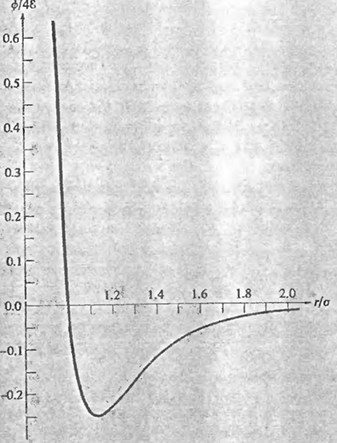
\includegraphics[width=0.4\textwidth]{images/7-Classificazione-Solidi/lennardjones.png}
    \caption{}
    \label{fig:lennard-jones}
\end{figure}
\begin{figure} [H]
    \centering
    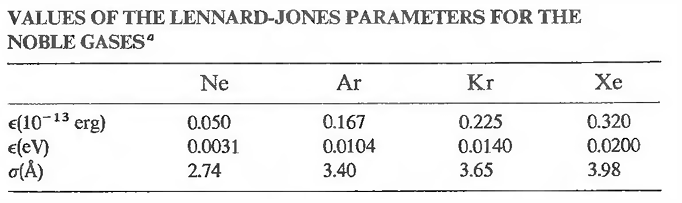
\includegraphics[width=0.75\textwidth]{images/7-Classificazione-Solidi/valori-lennard-jones.png}
    \caption{}
    \label{fig:valori-lennard-jones}
\end{figure}

Ora troviamo l'energia potenziale totale del solido. \\
L'energia di interazione totale di un atomo all'origine con tutti gli altri è data da:
\[ \sum_{\mathbf{R} \neq 0} \phi (\mathbf{R})\]
($R \neq 0$ perché non ho self interaction) \\
Quindi l'energia per singola particella è data da:
\begin{equation}
    u = \frac{1}{2} \sum_{\mathbf{R} \neq 0} \phi (\mathbf{R})
    \label{eqn:ulj}
\end{equation}
dove l'$1/2$ serve per evitare di contare 2 volte la stessa coppia di atomi. Quindi l'energia totale sarà quest'ultima per il numero N di particelle $\implies U = Nu$. \\
Conviene considerare R nel seguente modo:
\[ |\mathbf{R} | = \alpha(\mathbf{R}) r
\]
dove r è la distanza dell'atomo con i primi vicini e $\alpha(\mathbf{R})$ è un parametro che dipende dalla tipo di reticolo e ci dice che la posizione degli atomi è sempre nella stessa direzione nel solido. Quindi la (\ref{eqn:ulj}) inserendo (\ref{eqn:lennard-jones-pot}) con questo $R$ diventa:
\[ 
\begin{split}
&u = 2\varepsilon \left[ A_{12} \left( \frac{\sigma}{r}\right)^{12} - A_6 \left( \frac{\sigma}{r}\right)^6 \right] \\
&A_n = \sum_{R \neq 0} \frac{1}{\alpha(R)^n}
\end{split}
\]
$A_n$ è un termine che dipende quindi dal tipo di cristallo, alcuni valori sono riportati in Figura \ref{fig:valori-An}
\begin{figure} [H]
    \centering
    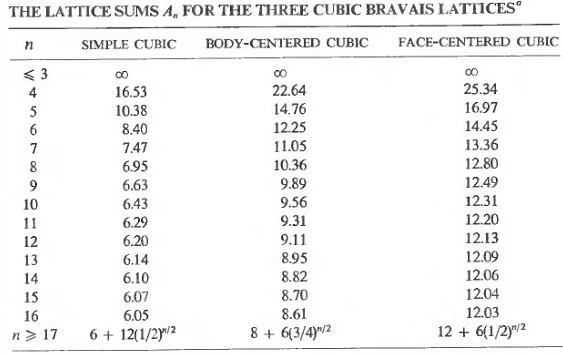
\includegraphics[width=0.75\textwidth]{images/7-Classificazione-Solidi/valoriAn.png}
    \caption{l'esponente deve essere maggiore di 3 altrimenti la serie non converge}
    \label{fig:valori-An}
\end{figure}

Posso trovare la distanza tra due atomi all'equilibrio facendo $\frac{\partial u}{\partial r} = 0$ e si ottiene
\[ r_0^{th} = \left( \frac{2A_{12}}{A_6} \right)^{\frac{1}{6}}\sigma = 1,09\sigma\]
Quindi all'equilibrio è:
\[ u_0^{th} = -\frac{\varepsilon A_6^2}{2A_{12}} = -8,6\varepsilon\]
Possiamo anche calcolare il \textbf{modulo di compressibilità} all'equilibrio che sarà dato da:
\[ \begin{split}
    &B = - V \left( \frac{\partial P}{\partial V}\right)_T \\
    & P = -\frac{dU}{dV}, \ \ v = \frac{V}{N} \\
    & B = v \frac{\partial}{\partial v}\left( \frac{\partial u}{\partial v}\right)_T
\end{split} \]
per un FCC (vedi Figura \ref{fig:FCC}) che ha lato di lunghezza $a$, la distanza di un atomo col suo primo vicino sarà data da $r$ ed è la diagonale di un quadrato di lato $a/2$. Perciò $a = \sqrt{2}r$ e ho 4 celle unitarie quindi:
\[v = \frac{a^3}{4} = \frac{r^3}{\sqrt{2}} \implies \frac{\partial }{\partial v} = \frac{\partial}{\partial r}\frac{\partial r}{\partial v} = \frac{\sqrt{2}}{3r^2}\frac{\partial}{\partial r}\]
B quindi diventa:
\[ B = \frac{r^3}{\sqrt{2}} \frac{\sqrt{2}}{3r^2} \frac{\partial}{\partial r} \frac{\sqrt{2}}{3r^2}\frac{\partial u}{\partial r} = \frac{\sqrt{2}}{9} r \frac{\partial}{\partial r}\frac{1}{r^2}\frac{\partial u}{\partial r}\]
se $r = r_0^{th} \equiv r_0$ abbiamo che 
\[ \begin{split}
     &B = \frac{\sqrt{2}}{9} r_0 \frac{\partial}{\partial r}\frac{1}{r_0^2}\frac{\partial u}{\partial r} = \frac{\sqrt{2}}{9} \frac{\cancel{r_0}}{r_0^{\cancel{2}}}\frac{\partial}{\partial r}\frac{\partial u}{\partial r} =\\
     & = \frac{\sqrt{2}}{9r_0}\left(\frac{\partial^2 u}{\partial r^2}\right)_{r=r_0} = \frac{4\varepsilon}{\sigma^3} A_{12} \left( \frac{A_6}{A_{12}} \right)^{\frac{5}{2}} = \frac{75\varepsilon}{\sigma^3}
    \end{split}\]

\subsection{Cristalli ionici}
Siccome un cristallo ionico è formato da ioni positivi e negativi che si alternano, ciascun ione sarà attratto da alcuni e respinto da altri in un suo intorno, perciò l'energia di coesione sarà data da due contributi: uno attrattiva coulombiano e uno repulsivo con i nuclei quando gli atomi si avvicinano troppo.
\[ u(r) = u^{\text{core}}(r) + u^{\text{coul}}(r) \]
Ci sarebbe anche da aggiungere il contributo delle forze di Van der Waals ma in questo caso sono trascurabili. \\\\
In questo caso $u^{\text{coul}}(r)$ è molto difficile da calcolare perché ho interazioni sia repulsive che attrattive. Considero l'esempio dell'\textbf{\ce{NaCl}} cristallo composto da 2 reticoli di Bravais FCC sovrapposti, uno composto da ioni negativi in posizione $\mathbf{R}$ e un secondo composto da ioni positivi spostato di \textbf{d} (vedi Figura \ref{fig:NaCl} e considera i pallini neri come ioni negativi e quelli bianchi come ioni positivi). \\
In un  FCC la distanza tra i primi vicini è data da $r = \frac{a}{2}$, quindi come prima si ottiene
\[ \begin{split} &|\mathbf{R}| = \alpha(R) r \ \ \ \  \text{reticolo fcc negativo} \\
& |\mathbf{R + d}| = \alpha(R+d) r \ \ \ \  \text{reticolo fcc positivo}
\end{split}
\]
Quindi il potenziale di un singolo anione o catione sarà:
\begin{equation}
    u^{\text{coul}}(r) = -\frac{e^2}{r} \left\{ \frac{1}{\alpha(d)} + \sum_{R \neq 0} \left( \frac{1}{\alpha(R + d)} - \frac{1}{\alpha(R)}\right)\right\}
    \label{eqn:ucoul}
\end{equation}
dove il primo termine è l'interazione attrattiva degli atomi all'interno di una cella, mentre tutto il resto è l'interazione con tutti gli altri ioni di tutte le altre celle. L'energia totale sarà
\[ U = - \frac{N}{2}\frac{e^2}{r} \left\{ \frac{1}{\alpha(d)} + \sum_{R \neq 0} \left( \frac{1}{\alpha(R + d)} - \frac{1}{\alpha(R)}\right)\right\}\]

\subsubsection{Costante di Madelung}
La (\ref{eqn:ucoul}) può essere scritta così:
\[ u^{\text{coul}}(r) = -\alpha_M \frac{e^2}{r}\]
Nel caso 1 dimensionale la situazione è la seguente:
\begin{figure} [H]
    \centering
    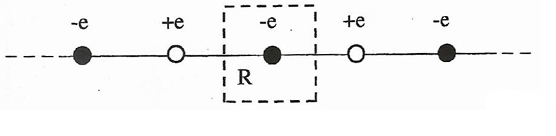
\includegraphics[width=0.75\textwidth]{images/7-Classificazione-Solidi/madel1d.png}
    \caption{}
    \label{fig:madel-1d}
\end{figure} 

Sviluppo la serie della (\ref{eqn:ucoul}) e diventa:
\[ u^{\text{coul}}(r) = - \frac{e^2}{2}2\left[\frac{1}{1}-\frac{1}{2}+\frac{1}{3}-\frac{1}{4}+\frac{1}{5}-...\right] = -\frac{e^2}{r}2\ln 2\]
Quindi la costante di Madelung è: $\alpha_M = 2 \ln 2$. Il numero 2 all'interno del logaritmo sta a indicare che le particelle coinvolte sono due. A dimensioni superiori l'interazione si fa più complicata e la serie potrebbe essere non ben definita e quindi divergere. \\
\textbf{L'idea di madelung è stata comprendere che la sommatoria dipende da come viene costruito il cristallo, introduce quindi delle interazioni quadrupolo suddividendo il cristallo in celle elettricamente neutre e a simmetria cubica nelle quali l'interazione elettrostatica cade rapidamente (come l'inverso della quinta potenza $\sim 1/r^5$) e in seguito calcola l'energia di interazione in ogni cella e tra le celle. }\\\\
Ogni cella contiene:\\
a)  4 unità di carica positiva composte da: $\frac{1}{1}$ una unità intera al centro e $\frac{12}{4}$ dodici quarti sui bordi \\
b)  4 unità di carica negativa composte da: $\frac{6}{2}$ sei metà (1 per ogni faccia) e $\frac{8}{8}$ otto ottavi sugli angoli, come in Figura \ref{fig:madel-3d}.
\begin{figure} [H]
    \centering
    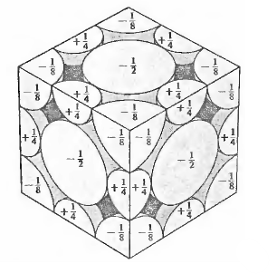
\includegraphics[width=0.4\textwidth]{images/7-Classificazione-Solidi/madel3d.png}
    \caption{}
    \label{fig:madel-3d}
\end{figure} 

Quindi l'interazione ora è divisa nell'interazione di una cella con tutte le altre e nell'interazione interna alla cella invece che l'atomo con tutti gli altri.\\
\[u = u_{\text{cell}}+u_{\text{int}}\]
La cella al suo interno ha delle interazioni di \textbf{quadrupolo} perché ho una carica centrale che interagisce con 4 cariche attorno. Quindi la serie diventa:
\[ u^{\text{coul}}(r) = -\frac{e^2}{r}\left[ \frac{6}{1}-\frac{12}{\sqrt{2}}+\frac{8}{\sqrt{3}}-\frac{3}{\sqrt{4}}+\frac{12}{\sqrt{5}}-\frac{12}{\sqrt{6}}-\frac{3}{\sqrt{8}}+\frac{6}{\sqrt{9}}-\frac{1}{\sqrt{12}}\right] = - 1,751 \frac{e^2}{r}\]
quindi $\alpha_M = 1,751$. \\
Siccome è poco diversa da 1 vuol dire che l'interazione con tutto il resto non è poi così importante, quasi tutta l'interazione coulombiana è ristretta alla cella elementare. 
\\~\\
Ora aggiungiamo a $u^{\text{coul}}(r)$ la repulsione dei nuclei che può essere rappresentata come qualcosa che varia rapidamente al variare della distanza tra gli ioni (la possiamo vedere come una correzione all'energia), quindi l'energia totale è:
\[ u(r) = - \frac{\alpha e^2}{r} + \frac{C}{r^m}\]
Per trovare la separazione all'equilibrio $r_0$ dobbiamo minimizzare $u(r)$ ponendo $\frac{\partial u}{\partial r} = 0$
\[ \begin{split}
    &r_0^{m-1} = \frac{mC}{e^2 \alpha} \implies C = \frac{\alpha e^2 r_o^{m-1}}{m} \\
    &u_0^{th} \equiv u(r_0) = -\frac{\alpha e^2}{r_0}\frac{m-1}{m} \\
    & m = 1 + \frac{18 B_0 r_0^3}{|u^{\text{coul}}(r_0)|}
    \end{split}
\]
dove $B_0$ è il modulo di compressibilità (bulk modulus). \\\\
\textbf{Dai valori riportati nella tabella in Figura \ref{fig:valori-ci} si nota che l'80\%-90\% dell'energia di coesione dei cristalli ionici è attrazione coulombiana, la correzione è veramente piccola.}
\begin{figure} [H]
    \centering
    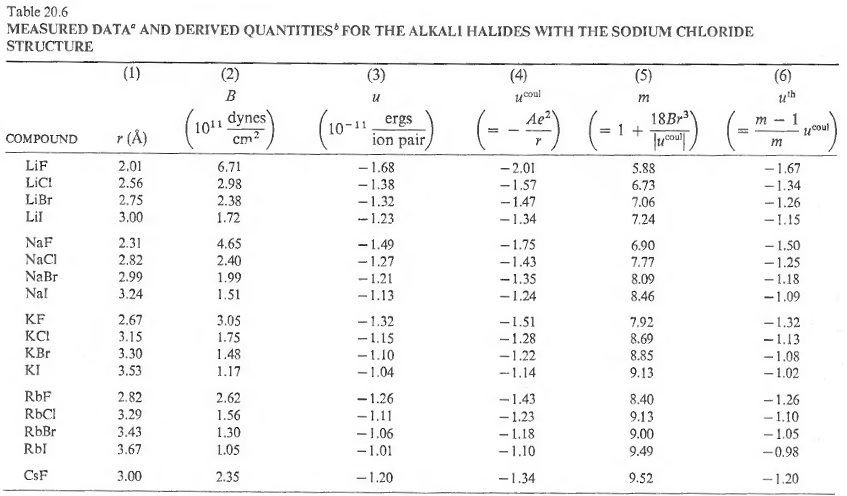
\includegraphics[width=\textwidth]{images/7-Classificazione-Solidi/valori-en-crist-ionici.png}
    \caption{}
    \label{fig:valori-ci}
\end{figure}

\subsection{Metalli}
Per i metali, ossia solidi ionici non covalenti, possiamo considerare un reticolo formato da ioni (positivi) fissi con una distribuzione degli elettroni di valenza uniforme su tutto il solido. \\
Quindi abbiamo che l'energia totale sarà data dalla somma dell'energia delle cariche puntiformi positive dei nuclei del metalle e dall'energia di un gas di elettroni con una densità di $\frac{3}{4}\pi r_s^3$ dove $r_s$ dipende dalla densità ed è dato da: $\frac{1}{n} = 4\pi r_s^3$, quindi 2 volte la distanza tra gli elettroni, e $n = \frac{N_e}{V}$ dove $N_e$ è il numero di elettroni di valenza.\\
Quindi l'energia totale è:
\[u^{\text{coul}} = - \frac{24.35}{(r_s/a_0)}  \ \ \ \text{eV/atomo}\]
L'energia è legata all'energia di Fermi $\varepsilon_F$, quindi calcoliamo l'energia cinetica:
\[ u^{\text{kin}} = \frac{3}{5}\varepsilon_F = \frac{30.1}{(r_s/a_0)^2} \ \ \text{eV/atomo}\]
è più alta dell'energia attrattiva quindi \textbf{c'è qualcosa che tiene il metallo stabile, questo significa che ci sono degli effetti quantistici e l'energia associata a questo è l'exchange energy}
\[ \begin{split}
    &u^{ex} = - \frac{12.5}{(r_s/a_0)} \ \ \text{eV/atomo} \\
    &\implies u = u^{kin} +u^{\text{coul}} + u^{ex} = \left[ \frac{30.1}{(r_s/a_0)^2} - \frac{24.35}{(r_s/a_0)} - \frac{12.5}{(r_s/a_0)} \right] \ \ \text{eV/atomo}  =\\
    & = \frac{30.1}{(r_s/a_0)^2} - \frac{36.8}{(r_s/a_0)} \ \ \text{eV/atomo} 
    \end{split}
\]
Minimizzando questa rispetto a $r_s$ troviamo:
\[ \frac{r_s}{a_0} = 1.6\]
